\documentclass[12pt, a4paper]{article}

% --- PACKAGES ---
\usepackage[T1]{fontenc}
\usepackage{microtype}
\usepackage{graphicx}
\usepackage{geometry}
\usepackage{hyperref}
\usepackage{titlesec}
\usepackage{xcolor}
\usepackage{mathpazo}
\usepackage[scaled]{helvet}
\usepackage{tocloft}
\usepackage{fancyhdr}
\usepackage{enumitem}
\usepackage{amssymb}
\usepackage{tcolorbox}
\usepackage{booktabs}
\usepackage{array}
\usepackage{longtable}
\usepackage{dirtree}
\tcbuselibrary{skins, breakable}
\usepackage{soul}

% --- COLORS (IsoCortex Theme) ---
\definecolor{ctPurple}{HTML}{311B5B}
\definecolor{ctGold}{HTML}{C59B47}
\definecolor{ctLightGold}{HTML}{FFF8E7}
\definecolor{ctLightPurple}{HTML}{F3E5F5}
\definecolor{alertRed}{HTML}{D32F2F}
\definecolor{ctGreen}{HTML}{1B5E20}
\definecolor{ctLightGreen}{HTML}{F1F8E9}

% --- GEOMETRY ---
\geometry{
    a4paper,
    total={170mm,257mm},
    left=25mm,
    right=25mm,
    top=25mm,
    bottom=30mm
}

% --- HYPERLINKS ---
\hypersetup{
    colorlinks=true,
    linkcolor=ctPurple,
    urlcolor=ctGold,
    pdftitle={IsoCortex SRS v2.0},
}

% --- SECTION STYLING ---
\titleformat{\section}
  {\normalfont\Large\bfseries\sffamily\color{ctPurple}}
  {\thesection}{1em}
  {}
  [{\color{ctGold}\titlerule[2pt]}]

\titleformat{\subsection}
  {\normalfont\large\bfseries\sffamily\color{ctPurple}}
  {\thesubsection}{1em}
  {}

% --- LIST STYLING ---
\newlist{prolist}{itemize}{3}
\setlist[prolist]{
    label=\textcolor{ctGold}{\tiny$\blacksquare$},
    leftmargin=*,
    itemsep=0.5em,
    topsep=0.5em
}

\newlist{trellolist}{enumerate}{1}
\setlist[trellolist]{
    label=\textbf{\textcolor{ctPurple}{\arabic*.}},
    leftmargin=*,
    itemsep=0.3em
}

% --- BOX STYLING ---
\tcbset{
    standardbox/.style={
        enhanced,
        colback=ctLightPurple,
        colframe=ctPurple,
        boxrule=0.5pt,
        leftrule=4pt,
        arc=3mm,
        boxsep=5pt,
        left=10pt,
        right=10pt,
        top=8pt,
        bottom=8pt,
        drop fuzzy shadow=black!10!white
    },
    alertbox/.style={
        enhanced,
        colback=red!5,
        colframe=alertRed,
        boxrule=1pt,
        leftrule=5pt,
        arc=3mm,
        fontupper=\itshape,
        drop fuzzy shadow=black!10!white
    },
    greenbox/.style={
        enhanced,
        colback=ctLightGreen,
        colframe=ctGreen,
        boxrule=0.5pt,
        leftrule=4pt,
        arc=3mm,
        drop fuzzy shadow=black!10!white
    }
}

% --- HEADER/FOOTER ---
\pagestyle{fancy}
\fancyhf{}
\fancyhead[R]{\footnotesize \textsf{\textbf{\textcolor{ctPurple}{Software Requirement Specification}}}}
\fancyhead[L]{\footnotesize \textsf{\textbf{\textcolor{ctPurple}{Iso}}\textbf{\textcolor{ctGold}{Cortex}}}}
\fancyfoot[C]{\textbf{\thepage}}
\renewcommand{\headrulewidth}{0.8pt}
\renewcommand{\headrule}{\hbox to\headwidth{\color{ctGold}\leaders\hrule height \headrulewidth\hfill}}

\begin{document}

% ======================================================================
% TITLE PAGE
% ======================================================================
\begin{titlepage}
    \centering
    \thispagestyle{empty}

    \noindent\makebox[\textwidth][l]{\hspace*{-25mm}{\color{ctPurple}\rule{\paperwidth}{8pt}}}

    \noindent
    \begin{minipage}[t]{0.5\textwidth}
        \vspace{0pt}
        {\Large \textsf{\textbf{\textcolor{ctPurple}{Project Documentation}}} \par}
        {\large \textsf{\textcolor{gray}{Architecture \& Requirements}} \par}
    \end{minipage}%
    \hfill
    \begin{minipage}[t]{0.4\textwidth}
        \vspace{0pt}
        \raggedleft
        {\large \textsf{\textcolor{gray}{Version 2.0}} \par}
        {\large \textsf{\textcolor{gray}{\today}} \par}
    \end{minipage}

    \vspace{2cm}

    
\includegraphics[width=0.45\textwidth]{logo.png}

    \vspace{1cm}

    \begin{tcolorbox}[standardbox, colback=ctLightGold, colframe=ctGold, leftrule=6pt]
        \centering
        {\Large \sffamily \textit{A High-Performance Localized Neural} \\ \textit{Information Retrieval Engine} \par}
    \end{tcolorbox}

    \vspace{0.7cm}

    {\Huge \textsf{\textbf{Software Requirement}} \par}
    {\Huge \textsf{\textbf{Specification (SRS)}} \par}

    \vspace{1.5cm}

    {\large \textbf{Lead Architect \& Developer:} \par}
    \vspace{0.2cm}
    {\Large \textbf{\textcolor{ctPurple}{Shaheer Qureshi}} \par}

    \vspace*{\fill}

    \noindent\makebox[\textwidth][l]{\hspace*{-25mm}{\color{ctGold}\rule{\paperwidth}{8pt}}}
\end{titlepage}

% ======================================================================
% TABLE OF CONTENTS
% ======================================================================
\newpage
\thispagestyle{empty}

\noindent\makebox[\textwidth][l]{\hspace*{-25mm}{\color{ctPurple}\rule{\paperwidth}{8pt}}}

\begingroup
\renewcommand{\cftsecfont}{\large\sffamily\bfseries\color{ctPurple}}
\renewcommand{\cftsubsecfont}{\sffamily\color{ctPurple!90}}
\renewcommand{\cftsecpagefont}{\large\sffamily\bfseries\color{ctGold}}
\renewcommand{\cftsubsecpagefont}{\sffamily\bfseries\color{ctGold}}
\renewcommand{\cftsecleader}{\color{ctGold}\cftdotfill{\cftdotsep}}
\renewcommand{\cftsubsecleader}{\color{ctGold!70}\cftdotfill{\cftdotsep}}
\setlength{\cftbeforesecskip}{1pt}

\begin{tcolorbox}[standardbox, breakable, colback=white, colframe=ctPurple,
    leftrule=4pt, rightrule=4pt, arc=4mm, top=15pt, bottom=15pt]
    \begin{center}
        {\Huge \sffamily \bfseries \color{ctPurple} \MakeUppercase{Table of Contents} \par}
        \vspace{0.3cm}
        {\color{ctGold}\rule{0.5\textwidth}{2pt}} \par
    \end{center}
    \renewcommand{\contentsname}{}
    \tableofcontents
\end{tcolorbox}
\endgroup

\vspace*{\fill}
\noindent\makebox[\textwidth][l]{\hspace*{-25mm}{\color{ctGold}\rule{\paperwidth}{8pt}}}
\newpage

% --- MAIN CONTENT STARTS HERE ---
\setcounter{page}{1}

% ======================================================================
% 1. INTRODUCTION & PROJECT OVERVIEW
% ======================================================================
\section{Introduction \& Project Overview}

\subsection{Problem Statement}

In the era of large language models and semantic search, businesses and
individuals face a critical dilemma when managing unstructured private data.
Current market solutions rely heavily on cloud-based vector databases
(e.g., Pinecone, Weaviate) and external embedding APIs (e.g., OpenAI).
This architecture introduces \textbf{severe limitations}:

\begin{tcolorbox}[standardbox, colback=white, colframe=ctPurple, leftrule=3pt]
\begin{prolist}
    \item \textbf{\textcolor{ctGold}{Data Privacy Risks:}} Uploading sensitive
    documents, proprietary source code, private archives, and confidential
    spreadsheets or presentations to third-party cloud servers violates strict
    confidentiality and compliance standards (e.g., GDPR, HIPAA, SOC~2).

    \item \textbf{\textcolor{ctGold}{Cost Overhead:}} Recurring subscription
    fees for cloud vector storage and token-based billing for embedding
    generation create prohibitive costs for local developers and small
    enterprises.

    \item \textbf{\textcolor{ctGold}{Network Latency \& Dependency:}} Relying
    on internet connectivity for semantic retrieval introduces latency and
    renders the system useless in offline or air-gapped environments.

    \item \textbf{\textcolor{ctGold}{Format Fragmentation:}} Enterprise
    knowledge is distributed across heterogeneous file formats---Word
    documents, PowerPoint decks, Excel spreadsheets, PDFs, and source
    code---with no unified local retrieval interface.
\end{prolist}
\end{tcolorbox}

\subsection{Project Purpose}

The purpose of \textbf{IsoCortex} is to provide a high-performance, 100\%
localized Neural Information Retrieval Engine that runs entirely on the
user's own machine---no installation as a system service, no background
daemon, and no network dependency of any kind. By coupling a flexible
Python ingestion pipeline with a custom C++ Hierarchical Navigable Small
World (HNSW) search engine, IsoCortex empowers users to perform semantic
searches across their private files---spanning the full spectrum of industry
file formats---with sub-millisecond latency, zero cloud dependencies, and
absolute data sovereignty.

IsoCortex is invoked directly from the command line as a \textbf{local
developer tool}: the user runs a Python script (or compiled binary) on
demand, and all processing terminates when the script exits.

\subsection{Scope}

IsoCortex is a backend engine and command-line software pipeline focused on
the extraction, embedding, and retrieval of unstructured data from a wide
array of industry-standard file formats. The system provides:

\begin{prolist}
    \item \textbf{Universal Directory Ingestion:} Parsing of local files
    across the following supported format categories:

    \vspace{0.4cm}
    \begin{tcolorbox}[greenbox, top=6pt, bottom=6pt]
    \small
    \begin{tabular}{@{} p{3.8cm} p{4.5cm} p{5.5cm} @{}}
        \toprule
        \textbf{\textcolor{ctGreen}{Category}}
            & \textbf{\textcolor{ctGreen}{Extensions}}
            & \textbf{\textcolor{ctGreen}{Library}} \\
        \midrule
        Plain Text
            & \texttt{.txt}, \texttt{.md}, \texttt{.log}
            & Built-in \texttt{open()} \\
        \addlinespace
        Source Code
            & \texttt{.py}, \texttt{.cpp}, \texttt{.js}, \texttt{.ts},
              \texttt{.java}, \texttt{.c}, \texttt{.h}
            & Built-in \texttt{open()} \\
        \addlinespace
        PDF Documents
            & \texttt{.pdf}
            & \texttt{pymupdf} (fitz) \\
        \addlinespace
        Word Documents
            & \texttt{.docx}, \texttt{.odt}
            & \texttt{python-docx} \\
        \addlinespace
        Presentations
            & \texttt{.pptx}, \texttt{.odp}
            & \texttt{python-pptx} \\
        \addlinespace
        Spreadsheets
            & \texttt{.xlsx}, \texttt{.xls}, \texttt{.ods}, \texttt{.csv}
            & \texttt{openpyxl} / \texttt{pandas} \\
        \addlinespace
        Email \& Web
            & \texttt{.eml}, \texttt{.html}, \texttt{.htm}
            & \texttt{email} / \texttt{BeautifulSoup4} \\
        \bottomrule
    \end{tabular}
    \end{tcolorbox}

    \item \textbf{Context-Aware Chunking:} Utilizing natural language
    processing to divide text into semantic nodes of $\sim$120 words with
    sentence-boundary awareness.

    \item \textbf{Structured Data Linearization:} Converting tabular data
    (spreadsheets) and slide-based content (presentations) into coherent
    natural-language text representations before chunking.

    \item \textbf{Local Vectorization:} Generating 384-dimensional dense
    vectors using the local \texttt{all-MiniLM-L6-v2} transformer model.

    \item \textbf{High-Speed Retrieval:} Executing logarithmic $O(\log N)$
    semantic searches via a C++ compiled core engine, bridged to Python via
    \texttt{pybind11}.
\end{prolist}

\subsection{Definitions \& Terminology}

\begin{tcolorbox}[standardbox, colback=white, colframe=ctPurple, leftrule=4pt]
\begin{prolist}
    \item \textbf{Embedding:} A numerical representation (vector) of text
    that captures its semantic meaning.

    \item \textbf{HNSW (Hierarchical Navigable Small World):} A
    state-of-the-art graph-based data structure that allows for rapid
    approximate nearest neighbour (ANN) search in high-dimensional spaces.

    \item \textbf{Cosine Similarity:} A mathematical metric used to measure
    how similar two document vectors are, regardless of their magnitude.

    \item \textbf{Context Window:} The maximum number of tokens an AI model
    can process at one time. For this project the limit is strictly
    256~tokens.

    \item \textbf{Linearization:} The process of converting structured or
    semi-structured data (e.g., spreadsheet rows, presentation slides) into
    a flat, readable natural-language string suitable for NLP chunking.

    \item \textbf{pybind11:} A lightweight C++11 header-only library that
    exposes C++ classes and functions as Python extension modules
    (\texttt{.so} on Linux/macOS, \texttt{.pyd} on Windows), enabling
    zero-copy in-process calls between Python and C++.

    \item \textbf{ANN (Approximate Nearest Neighbour):} A class of
    algorithms that find vectors \textit{approximately} closest to a query
    vector, trading marginal accuracy for dramatic speed gains.

    \item \textbf{efConstruction\,/\,efSearch:} HNSW tuning parameters
    controlling build-time graph quality and query-time search beam width,
    respectively.

    \item \textbf{Local Tool:} A program invoked manually by the user from
    the command line on their own machine. It has no persistent daemon
    process, no background service, and no installer.
\end{prolist}
\end{tcolorbox}

% ======================================================================
% 2. AGILE PROJECT MANAGEMENT (Trello Backlog)
% ======================================================================
\section{Agile Project Management \& Product Backlog}

To ensure rapid, iterative delivery, the development of IsoCortex is managed using the \textbf{Agile Scrum methodology}. All requirements, features, and bugs are tracked dynamically using a centralized Trello Kanban board.

\begin{tcolorbox}[standardbox, colback=ctLightGold, colframe=ctGold]
    \textbf{\textcolor{ctPurple}{Project Tracking:}} \\
    The development lifecycle is tracked via a live Scrum board, ensuring transparent progression from architectural planning to C++ implementation and Python integration.
\end{tcolorbox}

\noindent The board is strictly organized into the following \textbf{Pipeline} to track the lifecycle of every feature:

\vspace{0.3cm}
\begin{tcolorbox}[standardbox, colback=ctLightPurple, colframe=ctPurple]
\begin{trellolist}
    \item \textbf{Assets:} Design files, models, architecture diagrams, and SRS documents.
    \item \textbf{Product Backlog:} The master list of all approved FRs and NFRs (Epics \& User Stories).
    \item \textbf{Sprint Backlog:} Tasks selected for the current active development sprint (e.g., C++ graph logic).
    \item \textbf{Sprint Dev in Progress:} Tasks actively being coded by the engineering team.
    \item \textbf{Sprint Dev Completed:} Code is written but pending quality assurance.
    \item \textbf{Sprint QA in Progress:} Active testing (unit testing, C++ memory leak checks, Python integration checks).
    \item \textbf{Bugs:} Any defects identified during QA that require developer remediation.
    \item \textbf{Completed:} Feature successfully merged into the `main` branch.
\end{trellolist}
\end{tcolorbox}

% ======================================================================
% 3. SYSTEM ARCHITECTURE
% ======================================================================
\section{System Architecture}

IsoCortex is a \textbf{locally executed, on-demand command-line tool}. It
does not run as a background service or system daemon. All processing
begins when the user invokes a command and terminates when that command
completes. It utilises a \textbf{Two-Tier Local Processing Pipeline},
isolating high-level natural language processing tasks from low-level
memory management and search execution.

\begin{tcolorbox}[standardbox, colback=ctLightGold, colframe=ctGold]
    \textbf{\textcolor{ctPurple}{Layer 1: The Python Ingestion Engine
    (The Sensory Input)}} \\[4pt]
    Responsible for recursive directory scanning, format-specific text
    extraction, structured data linearization, semantic chunking, and model
    inference. Python is chosen for its superior ecosystem of document
    parsing and machine learning libraries (e.g.,
    \texttt{sentence-transformers}, \texttt{python-docx},
    \texttt{python-pptx}, \texttt{openpyxl}, \texttt{pymupdf}).
\end{tcolorbox}

\vspace{0.3cm}

\begin{tcolorbox}[standardbox, colback=ctLightPurple, colframe=ctPurple]
    \textbf{\textcolor{ctGold}{Layer 2: The C++ HNSW Core
    (The Gray Matter)}} \\[4pt]
    Responsible for ingesting the exported binary vector data, constructing
    the multi-layered HNSW graph in RAM, executing Cosine Similarity
    mathematical operations, and persisting the index to disk. C++ is
    utilised to ensure optimal memory allocation and sub-millisecond
    retrieval speeds. The C++ core is compiled as a native Python extension
    module via \texttt{pybind11}, enabling in-process, zero-file-I/O query
    execution at runtime without any separate server or daemon.
\end{tcolorbox}

\vspace{0.5cm}
\subsubsection*{\textsf{\textcolor{ctPurple}{HNSW Tuning Parameters}}}
\vspace{0.2cm}

The following parameters govern the quality-vs-performance trade-off of the
HNSW graph and \textbf{must be exposed as configurable values} via
\texttt{config.json}:

\begin{tcolorbox}[standardbox, colback=white, colframe=ctPurple, leftrule=4pt]
\begin{center}
\small
\begin{tabular}{@{} l p{6.2cm} c c @{}}
    \toprule
    \textbf{Parameter} & \textbf{Role} & \textbf{Default} & \textbf{Tunable} \\
    \midrule
    \texttt{M}
        & Max edges per graph node; controls connectivity
        & \texttt{16} & Yes \\
    \addlinespace
    \texttt{efConstruction}
        & Build-time beam width; higher = better graph, slower build
        & \texttt{200} & Yes \\
    \addlinespace
    \texttt{efSearch}
        & Query-time beam width; higher = better recall, slower search
        & \texttt{50} & Yes \\
    \addlinespace
    \texttt{dim}
        & Vector dimensionality (fixed by model)
        & \texttt{384} & No \\
    \addlinespace
    \texttt{space}
        & Distance metric (\texttt{cosine} or \texttt{l2})
        & \texttt{cosine} & Yes \\
    \bottomrule
\end{tabular}
\end{center}
\end{tcolorbox}

\vspace{0.5cm}
\subsubsection*{\textsf{\textcolor{ctPurple}{Technology Stack}}}
\vspace{0.2cm}

\begin{tcolorbox}[standardbox, colback=white, colframe=ctPurple, leftrule=4pt]
\begin{center}
\small
\begin{tabular}{@{} l l p{5.2cm} @{}}
    \toprule
    \textbf{Concern} & \textbf{Library / Tool} & \textbf{Rationale} \\
    \midrule
    PDF extraction
        & \texttt{pymupdf} (fitz)
        & Fastest, most robust; handles complex layouts \\
    \addlinespace
    Word extraction
        & \texttt{python-docx}
        & Official OOXML support for \texttt{.docx} \\
    \addlinespace
    Presentation extraction
        & \texttt{python-pptx}
        & Official OOXML support for \texttt{.pptx} \\
    \addlinespace
    Spreadsheet extraction
        & \texttt{openpyxl} / \texttt{pandas}
        & Structure access + row linearization \\
    \addlinespace
    Web/Email extraction
        & \texttt{BeautifulSoup4} / \texttt{email}
        & HTML tag stripping; RFC~5322 email parsing \\
    \addlinespace
    Sentence boundary
        & \texttt{spacy} (\texttt{en\_core\_web\_sm})
        & Accurate sentence tokenization for FR-2 \\
    \addlinespace
    Token counting
        & \texttt{transformers.AutoTokenizer}
        & Exact sub-word token count for NFR-2 \\
    \addlinespace
    Embedding model
        & \texttt{sentence-transformers}
        & Local CPU/GPU inference, 384-dim output \\
    \addlinespace
    C++ bridge
        & \texttt{pybind11}
        & Zero-copy NumPy array handoff to C++ \\
    \addlinespace
    Build system
        & \texttt{CMake} $\geq$ 3.15
        & Compiles C++ extension; no installer needed \\
    \addlinespace
    Unit testing (Python)
        & \texttt{pytest}
        & FR validation, chunking correctness \\
    \addlinespace
    Unit testing (C++)
        & \texttt{GoogleTest}
        & HNSW correctness, recall benchmarks \\
    \bottomrule
\end{tabular}
\end{center}
\end{tcolorbox}

\vspace{0.5cm}
\subsubsection*{\textsf{\textcolor{ctPurple}{Recommended Project Structure}}}
\vspace{0.2cm}

\begin{tcolorbox}[standardbox, colback=white, colframe=ctPurple, leftrule=4pt]
\small
\dirtree{%
.1 isocortex/.
.2 ingestion/.
.3 scanner.py \DTcomment{FR-1: Recursive directory scan}.
.3 extractor.py \DTcomment{FR-1: Format-specific text extraction}.
.3 chunker.py \DTcomment{FR-2: Sentence-aware chunking w/ overlap}.
.3 embedder.py \DTcomment{FR-3: all-MiniLM-L6-v2 inference}.
.2 export/.
.3 serializer.py \DTcomment{FR-4: .bin + metadata JSON export}.
.2 core/.
.3 hnsw.hpp \DTcomment{HNSW graph data structure}.
.3 hnsw.cpp \DTcomment{Graph construction and search}.
.3 cosine.hpp \DTcomment{Cosine similarity (SIMD-optimized)}.
.3 persist.cpp \DTcomment{FR-7: Index save/load}.
.3 bindings.cpp \DTcomment{FR-8: pybind11 Python bindings}.
.2 cli/.
.3 main.py \DTcomment{UC-1, UC-2, UC-3: CLI entry point}.
.2 tests/.
.3 test\_chunker.py \DTcomment{NFR-5: Chunking unit tests}.
.3 test\_extractor.py \DTcomment{NFR-5: Format extraction unit tests}.
.3 test\_search.cpp \DTcomment{NFR-6: HNSW recall benchmarks}.
.2 config.json \DTcomment{HNSW tuning parameters}.
.2 CMakeLists.txt.
.2 requirements.txt.
.2 README.md.
}
\end{tcolorbox}

% ======================================================================
% 4. FUNCTIONAL REQUIREMENTS
% ======================================================================
\section{Functional Requirements}

\subsection{Data Extraction \& Chunking}
\vspace{0.3cm}

\begin{tcolorbox}[enhanced, colback=white, colframe=ctPurple,
    colbacktitle=ctLightPurple, coltitle=ctPurple, boxrule=0.5pt,
    leftrule=4pt, arc=2mm, fonttitle=\large\bfseries,
    title={FR-1: Bulk Directory Ingestion},
    drop fuzzy shadow=black!5!white, top=2pt, bottom=2pt]
\begin{prolist}
    \item \textbf{Description:} The Python pipeline shall accept a root
    directory path, recursively traverse all subdirectories, and identify
    all supported file types as defined in Section~1.3.

    \item \textbf{Inputs:} Local file-system path string provided as a
    command-line argument.

    \item \textbf{Outputs:} Extracted raw text strings and associated
    metadata (file name, absolute path, format type, sheet/slide index
    where applicable).

    \item \textbf{Supported Formats:} \texttt{.txt}, \texttt{.md},
    \texttt{.log}, \texttt{.py}, \texttt{.cpp}, \texttt{.js}, \texttt{.ts},
    \texttt{.java}, \texttt{.c}, \texttt{.h}, \texttt{.pdf}, \texttt{.docx},
    \texttt{.odt}, \texttt{.pptx}, \texttt{.odp}, \texttt{.xlsx},
    \texttt{.xls}, \texttt{.ods}, \texttt{.csv}, \texttt{.eml},
    \texttt{.html}, \texttt{.htm}.

    \item \textbf{Priority:} \textcolor{alertRed}{\textbf{High}}
\end{prolist}
\end{tcolorbox}

\vspace{0.4cm}

\begin{tcolorbox}[enhanced, colback=white, colframe=ctPurple,
    colbacktitle=ctLightPurple, coltitle=ctPurple, boxrule=0.5pt,
    leftrule=4pt, arc=2mm, fonttitle=\large\bfseries,
    title={FR-1b: Structured Data Linearization},
    drop fuzzy shadow=black!5!white, top=2pt, bottom=2pt]
\begin{prolist}
    \item \textbf{Description:} For structured or semi-structured file
    formats, the Python pipeline shall convert content into coherent
    natural-language strings prior to chunking, as follows:
    \begin{prolist}
        \item \textbf{Spreadsheets} (\texttt{.xlsx}, \texttt{.xls},
        \texttt{.ods}, \texttt{.csv}): Each row shall be linearized as a
        key-value string using column headers as keys
        (e.g., \textit{``Name: Alice \textbar{} Department: Engineering
        \textbar{} Salary: 85000''}). Each sheet is processed independently
        and identified by its sheet name in the metadata.

        \item \textbf{Presentations} (\texttt{.pptx}, \texttt{.odp}): Text
        shall be extracted from all shapes, text boxes, and placeholders per
        slide. Each slide's content is prefixed with its slide number for
        traceability
        (e.g., \textit{``[Slide~3] Q2 Revenue grew by 24\% year-on-year%
        \ldots''}).

        \item \textbf{Word Documents} (\texttt{.docx}, \texttt{.odt}): Text
        shall be extracted paragraph-by-paragraph, preserving heading
        hierarchy as inline labels.

        \item \textbf{Email} (\texttt{.eml}): Subject, sender, date, and
        decoded body shall be extracted and concatenated into a single
        document string.

        \item \textbf{HTML\,/\,Web} (\texttt{.html}, \texttt{.htm}):
        Boilerplate tags, scripts, and styling shall be stripped; only
        semantic body text shall be retained.
    \end{prolist}

    \item \textbf{Outputs:} A normalised plain-text string per document (or
    per sheet/slide) ready for the chunking stage.

    \item \textbf{Priority:} \textcolor{alertRed}{\textbf{High}}
\end{prolist}
\end{tcolorbox}

\vspace{0.4cm}

\begin{tcolorbox}[enhanced, colback=white, colframe=ctPurple,
    colbacktitle=ctLightPurple, coltitle=ctPurple, boxrule=0.5pt,
    leftrule=4pt, arc=2mm, fonttitle=\large\bfseries,
    title={FR-2: Sentence-Aware Chunking},
    drop fuzzy shadow=black!5!white, top=2pt, bottom=2pt]
\begin{prolist}
    \item \textbf{Description:} The system shall partition extracted text
    into segments of approximately 120~words. The split must occur at the
    nearest natural sentence boundary (e.g., period or newline) to preserve
    semantic meaning.

    \item \textbf{Overlap Constraint:} The system must enforce a 25--30\%
    word overlap (approx.\ 30~words) between consecutive chunks to maintain
    contextual continuity.

    \item \textbf{Token Guard:} Before each chunk is passed to the embedding
    model, its sub-word token count shall be verified via
    \texttt{transformers.AutoTokenizer}. Any chunk exceeding 256~tokens must
    be further split automatically to comply with NFR-2.

    \item \textbf{Priority:} \textcolor{alertRed}{\textbf{High}}
\end{prolist}
\end{tcolorbox}

\vspace{0.5cm}
\subsection{Vectorization \& Handoff}
\vspace{0.3cm}

\begin{tcolorbox}[enhanced, colback=white, colframe=ctPurple,
    colbacktitle=ctLightPurple, coltitle=ctPurple, boxrule=0.5pt,
    leftrule=4pt, arc=2mm, fonttitle=\large\bfseries,
    title={FR-3: Local Neural Embedding},
    drop fuzzy shadow=black!5!white, top=2pt, bottom=2pt]
\begin{prolist}
    \item \textbf{Description:} The Python engine shall process every text
    chunk through the locally stored \texttt{all-MiniLM-L6-v2} transformer
    model using \texttt{sentence-transformers}. Inference must run entirely
    on the local CPU or GPU; no network calls are permitted at any stage.

    \item \textbf{Outputs:} A 384-dimensional dense floating-point vector
    for each chunk.

    \item \textbf{Batching:} Chunks shall be processed in configurable
    batches (default: 64) to maximise CPU/GPU throughput.

    \item \textbf{Priority:} \textcolor{alertRed}{\textbf{High}}
\end{prolist}
\end{tcolorbox}

\vspace{0.4cm}

\begin{tcolorbox}[enhanced, colback=white, colframe=ctPurple,
    colbacktitle=ctLightPurple, coltitle=ctPurple, boxrule=0.5pt,
    leftrule=4pt, arc=2mm, fonttitle=\large\bfseries,
    title={FR-4: Interoperability Export},
    drop fuzzy shadow=black!5!white, top=2pt, bottom=2pt]
\begin{prolist}
    \item \textbf{Description:} The Python pipeline shall serialise the
    vector matrix and text metadata to disk after each ingestion run.
    \textbf{CSV is explicitly prohibited} due to floating-point precision
    loss and excessive file size.

    \item \textbf{Required Format:} A flat binary \texttt{.bin} file
    structured as:
    \texttt{[n\_vectors:\,uint32][dim:\,uint32]%
    [vectors:\,float32\,$\times$\,n\,$\times$\,dim]},
    accompanied by a co-located \texttt{metadata.json} sidecar containing
    chunk ID, source file path, format type, sheet/slide index, and raw
    chunk text.

    \item \textbf{Alternate Format:} NumPy \texttt{.npy} files are an
    acceptable alternative for the vector matrix during development, given
    their lossless precision and trivial C++ interoperability via memory
    mapping.

    \item \textbf{Outputs:} Two files written to a configurable output
    directory: \texttt{vectors.bin} (or \texttt{vectors.npy}) and
    \texttt{metadata.json}.

    \item \textbf{Priority:} \textcolor{ctGold}{\textbf{Medium}}
\end{prolist}
\end{tcolorbox}

\vspace{0.5cm}
\subsection{Search Execution (C++ Core)}
\vspace{0.3cm}

\begin{tcolorbox}[enhanced, colback=white, colframe=ctPurple,
    colbacktitle=ctLightPurple, coltitle=ctPurple, boxrule=0.5pt,
    leftrule=4pt, arc=2mm, fonttitle=\large\bfseries,
    title={FR-5: HNSW Graph Construction},
    drop fuzzy shadow=black!5!white, top=2pt, bottom=2pt]
\begin{prolist}
    \item \textbf{Description:} The C++ engine shall read the exported
    binary vector file and construct an in-memory multi-layered HNSW graph
    using the configurable parameters defined in Section~3
    (\texttt{M}, \texttt{efConstruction}, \texttt{dim}, \texttt{space}).

    \item \textbf{Error Handling:} If the binary file is malformed or the
    declared vector dimensionality does not equal~384, the engine shall emit
    a structured error message to \texttt{stderr} and halt gracefully.

    \item \textbf{Priority:} \textcolor{alertRed}{\textbf{High}}
\end{prolist}
\end{tcolorbox}

\vspace{0.4cm}

\begin{tcolorbox}[enhanced, colback=white, colframe=ctPurple,
    colbacktitle=ctLightPurple, coltitle=ctPurple, boxrule=0.5pt,
    leftrule=4pt, arc=2mm, fonttitle=\large\bfseries,
    title={FR-6: Semantic Query Execution},
    drop fuzzy shadow=black!5!white, top=2pt, bottom=2pt]
\begin{prolist}
    \item \textbf{Description:} The system shall accept a natural language
    query string, vectorize it using the locally loaded embedding model, and
    pass the resulting 384-dimensional vector to the C++ core via
    \texttt{pybind11} bindings (zero file I/O at query time). The C++ core
    will return the top-$K$ most relevant document chunks based on Cosine
    Similarity scoring, where $K$ is configurable.

    \item \textbf{Outputs:} A ranked list of relevant text chunks, their
    Cosine Similarity scores, and their source file paths (including
    sheet/slide index for structured formats), printed to \texttt{stdout}.

    \item \textbf{Priority:} \textcolor{alertRed}{\textbf{High}}
\end{prolist}
\end{tcolorbox}

\vspace{0.4cm}

\begin{tcolorbox}[enhanced, colback=white, colframe=ctPurple,
    colbacktitle=ctLightPurple, coltitle=ctPurple, boxrule=0.5pt,
    leftrule=4pt, arc=2mm, fonttitle=\large\bfseries,
    title={FR-7: Index Persistence},
    drop fuzzy shadow=black!5!white, top=2pt, bottom=2pt]
\begin{prolist}
    \item \textbf{Description:} The C++ engine shall serialise the fully
    constructed HNSW graph to a binary index file on disk
    (e.g., \texttt{isocortex.index}). On subsequent invocations of the
    search command, the engine shall reload the saved index from disk
    without requiring re-ingestion of source documents.

    \item \textbf{Outputs:} A persistent binary index file written to a
    configurable path on the local file system.

    \item \textbf{Incremental Insertion:} If new documents are ingested, the
    system shall support inserting new nodes into the existing in-memory
    index without requiring a full rebuild, where algorithmically feasible,
    before re-saving to disk.

    \item \textbf{Priority:} \textcolor{alertRed}{\textbf{High}}
\end{prolist}
\end{tcolorbox}

\vspace{0.4cm}

\begin{tcolorbox}[enhanced, colback=white, colframe=ctPurple,
    colbacktitle=ctLightPurple, coltitle=ctPurple, boxrule=0.5pt,
    leftrule=4pt, arc=2mm, fonttitle=\large\bfseries,
    title={FR-8: Python--C++ Runtime Bridge},
    drop fuzzy shadow=black!5!white, top=2pt, bottom=2pt]
\begin{prolist}
    \item \textbf{Description:} The C++ HNSW engine shall be compiled as a
    native Python extension module using \texttt{pybind11}. The compiled
    \texttt{.so} (Linux/macOS) or \texttt{.pyd} (Windows) file is placed in
    the \texttt{core/} directory and imported directly by the Python
    scripts---no system-wide installation is required. The module shall
    expose at minimum the following interface:
    \begin{prolist}
        \item \texttt{build\_index(vectors: np.ndarray, config: dict)
              \textrightarrow{} None}
        \item \texttt{save\_index(path: str)
              \textrightarrow{} None}
        \item \texttt{load\_index(path: str)
              \textrightarrow{} None}
        \item \texttt{search(query\_vector: np.ndarray, k: int)
              \textrightarrow{} List[Tuple[int, float]]}
    \end{prolist}

    \item \textbf{Zero-Copy Constraint:} Vector data shall be transferred as
    \texttt{float32} NumPy arrays using \texttt{pybind11}'s buffer protocol
    to eliminate serialisation overhead.

    \item \textbf{Build:} The extension is compiled once by the developer
    via \texttt{cmake -{-}build build/} from the project root. The resulting
    module file is used in-place; no package manager or system-wide
    installation step is needed.

    \item \textbf{Priority:} \textcolor{alertRed}{\textbf{High}}
\end{prolist}
\end{tcolorbox}

% ======================================================================
% 5. NON-FUNCTIONAL REQUIREMENTS
% ======================================================================
\section{Non-Functional Requirements}

\subsection{Performance \& Efficiency}

\begin{tcolorbox}[enhanced, colback=white, colframe=ctGold,
    colbacktitle=ctLightGold, coltitle=ctPurple, boxrule=0.5pt,
    leftrule=4pt, arc=2mm, fonttitle=\large\bfseries,
    title={NFR-1: Retrieval Latency},
    drop fuzzy shadow=black!5!white]
\begin{prolist}
    \item \textbf{Description:} Once the HNSW graph is loaded into RAM, the
    C++ search execution (FR-6) must achieve sub-millisecond retrieval
    speeds for single-query execution on an index of up to 100,000~vectors.

    \item \textbf{Measurability:} Benchmarked via internal C++
    \texttt{std::chrono} timer modules; query execution time is appended to
    \texttt{benchmark.log} in the project directory.
\end{prolist}
\end{tcolorbox}

\begin{tcolorbox}[enhanced, colback=white, colframe=ctGold,
    colbacktitle=ctLightGold, coltitle=ctPurple, boxrule=0.5pt,
    leftrule=4pt, arc=2mm, fonttitle=\large\bfseries,
    title={NFR-2: Context Integrity},
    drop fuzzy shadow=black!5!white]
\begin{prolist}
    \item \textbf{Description:} Zero text truncation is permitted. The
    chunking algorithm (FR-2) must guarantee that no generated segment
    exceeds the 256-token limit of the \texttt{all-MiniLM-L6-v2} model.
    This applies equally to chunks derived from all supported file formats,
    including linearized spreadsheet rows and slide text.

    \item \textbf{Measurability:} Enforced by the token guard in FR-2;
    violations are logged as \texttt{[ERROR]} to \texttt{stderr} and the
    offending chunk is re-split automatically before being passed to the
    embedding model.
\end{prolist}
\end{tcolorbox}

\subsection{Security \& Operations}

\begin{tcolorbox}[enhanced, colback=white, colframe=ctGold,
    colbacktitle=ctLightGold, coltitle=ctPurple, boxrule=0.5pt,
    leftrule=4pt, arc=2mm, fonttitle=\large\bfseries,
    title={NFR-3: Absolute Privacy (Air-Gapped Operation)},
    drop fuzzy shadow=black!5!white]
\begin{prolist}
    \item \textbf{Description:} 100\% of data processing---including format
    extraction, linearization, model inference, and graph searching---must
    occur locally on the host machine. The system must not make any outbound
    network requests at any point during ingestion, indexing, or querying.
    This is enforced by design: the tool has no network client code and all
    model weights are loaded from the local file system.

    \item \textbf{Verification:} All third-party Python libraries must be
    pinned to specific versions in \texttt{requirements.txt} and installed
    into a local virtual environment (\texttt{venv}) from a local package
    cache where required for air-gapped deployment.
\end{prolist}
\end{tcolorbox}

\begin{tcolorbox}[enhanced, colback=white, colframe=ctGold,
    colbacktitle=ctLightGold, coltitle=ctPurple, boxrule=0.5pt,
    leftrule=4pt, arc=2mm, fonttitle=\large\bfseries,
    title={NFR-4: Zero Operational Cost},
    drop fuzzy shadow=black!5!white]
\begin{prolist}
    \item \textbf{Description:} The architecture must completely bypass
    commercial APIs, ensuring a \$0 recurring operational cost for the
    end-user. All libraries used must be open-source with permissive
    licences (MIT, Apache~2.0, or BSD).
\end{prolist}
\end{tcolorbox}

\subsection{Quality \& Testing}

\begin{tcolorbox}[enhanced, colback=white, colframe=ctGold,
    colbacktitle=ctLightGold, coltitle=ctPurple, boxrule=0.5pt,
    leftrule=4pt, arc=2mm, fonttitle=\large\bfseries,
    title={NFR-5: Unit \& Integration Testing},
    drop fuzzy shadow=black!5!white]
\begin{prolist}
    \item \textbf{Description:} The system shall include automated tests
    covering:
    \begin{prolist}
        \item \textbf{Chunking correctness (Python / pytest):} Verify
        overlap percentage, sentence-boundary respect, and token-count
        compliance for all supported format outputs.

        \item \textbf{Format extraction (Python / pytest):} Verify correct
        text extraction from sample \texttt{.docx}, \texttt{.pptx},
        \texttt{.xlsx}, \texttt{.csv}, \texttt{.pdf}, and \texttt{.eml}
        fixture files stored in \texttt{tests/fixtures/}.

        \item \textbf{C++ HNSW correctness (GoogleTest):} Verify graph
        construction, serialisation/deserialisation round-trips, and search
        result validity on a known toy dataset.
    \end{prolist}

    \item \textbf{Execution:} Tests are run locally via
    \texttt{pytest tests/} (Python) and \texttt{ctest} (C++) from the
    project root. No CI server is required for MVP.

    \item \textbf{Priority:} \textcolor{ctGold}{\textbf{Medium}}
\end{prolist}
\end{tcolorbox}

\begin{tcolorbox}[enhanced, colback=white, colframe=ctGold,
    colbacktitle=ctLightGold, coltitle=ctPurple, boxrule=0.5pt,
    leftrule=4pt, arc=2mm, fonttitle=\large\bfseries,
    title={NFR-6: HNSW Recall Benchmarks},
    drop fuzzy shadow=black!5!white]
\begin{prolist}
    \item \textbf{Description:} The C++ HNSW search shall achieve a minimum
    \textbf{Recall@10 of 95\%} as measured against brute-force exact
    nearest-neighbour results on a representative 10,000-vector benchmark
    dataset.

    \item \textbf{Measurability:} The benchmark script
    \texttt{tests/test\_search.cpp} generates ground truth via an exhaustive
    cosine scan and compares it against HNSW results, printing a recall
    report to \texttt{stdout}.

    \item \textbf{Priority:} \textcolor{ctGold}{\textbf{Medium}}
\end{prolist}
\end{tcolorbox}

\begin{tcolorbox}[enhanced, colback=white, colframe=ctGold,
    colbacktitle=ctLightGold, coltitle=ctPurple, boxrule=0.5pt,
    leftrule=4pt, arc=2mm, fonttitle=\large\bfseries,
    title={NFR-7: Index Build Latency},
    drop fuzzy shadow=black!5!white]
\begin{prolist}
    \item \textbf{Description:} HNSW graph construction time shall be
    measured and reported to the terminal upon completion of the index
    command. Target: build an index of 10,000~vectors in under 30~seconds
    on a commodity CPU (e.g., Intel Core~i5, 8~GB RAM).

    \item \textbf{Measurability:} Build duration measured via
    \texttt{std::chrono} and reported as:
    \texttt{[IsoCortex] Index built: N vectors in X.XXs}.

    \item \textbf{Priority:} \textcolor{ctGold}{\textbf{Low}}
\end{prolist}
\end{tcolorbox}

% ======================================================================
% 6. INTERFACE & DOMAIN REQUIREMENTS
% ======================================================================
\newpage
\section{Interface \& Domain Requirements}

\subsection{Interface Requirements}
\begin{tcolorbox}[standardbox, colback=white, colframe=ctPurple, leftrule=4pt]
\begin{prolist}
    \item \textbf{UI-1: Command Line Interface (CLI):} The primary interface for IsoCortex shall be a terminal-based CLI executed via Python (`python cli/main.py`). It must support distinct operational commands (e.g., `index`, `search`) and robust argument parsing.
    \item \textbf{API-1: C++ Runtime Bridge:} The C++ engine must be strictly wrapped using `pybind11` to allow Python to call graph construction and search functions directly without executing external binary subprocesses.
    \item \textbf{HW-1: Local Hardware Execution:} The system must run entirely on the user's local CPU (or local CUDA-enabled GPU if configured). It requires local read/write permissions for the target directories and the internal `isocortex.index` file.
\end{prolist}
\end{tcolorbox}

\subsection{Domain Requirements}
\begin{tcolorbox}[standardbox, colback=white, colframe=ctPurple, leftrule=4pt]
\begin{prolist}
    \item \textbf{DR-1: Operating System Agnosticism:} The Python pipeline and C++ CMake build system must be cross-platform, capable of running on Windows, macOS, and Linux environments without requiring OS-specific source code modifications.
    \item \textbf{DR-2: File Permission Respect:} The ingestion scanner must gracefully handle read-only files and directory permission errors without crashing the global indexing process.
\end{prolist}
\end{tcolorbox}

% ======================================================================
% 7. USE CASES & USER STORIES
% ======================================================================
\section{Use Cases \& User Stories}

\subsection{Use Cases}

\begin{tcolorbox}[enhanced, colback=white, colframe=ctPurple,
    colbacktitle=ctLightPurple, coltitle=ctPurple, boxrule=0.5pt,
    leftrule=4pt, arc=2mm, fonttitle=\large\bfseries,
    title={UC-1: Indexing a Local Directory},
    drop fuzzy shadow=black!5!white, top=2pt, bottom=2pt]
\textbf{Actor:} User (developer / analyst operating the local machine) \\[4pt]
\textbf{Trigger:} User executes the index script from a terminal. \\[4pt]
\textbf{Main Flow:}
\begin{trellolist}
    \item User opens a terminal and runs:
    \texttt{python cli/main.py index ./my\_documents}
    \item The Python ingestion engine recursively scans the directory,
    identifying all supported file types.
    \item Format-specific extractors parse each file; structured formats
    (spreadsheets, presentations) are linearized into natural-language
    strings.
    \item The text is chunked with sentence-boundary enforcement and
    enforced overlap; each chunk is token-validated before embedding.
    \item All chunks are vectorized in batches via the locally loaded
    \texttt{all-MiniLM-L6-v2} model.
    \item The vector matrix and metadata sidecar are written to
    \texttt{vectors.bin} and \texttt{metadata.json} in the configured
    output directory.
    \item The C++ engine (loaded via \texttt{pybind11}) reads the binary
    file, constructs the HNSW graph in RAM, and saves the persistent index
    to \texttt{isocortex.index}.
    \item The terminal reports:\\
    \texttt{[IsoCortex] Indexed N chunks from M files in X.Xs.}
\end{trellolist}
\textbf{Alternate Flow:} If an unsupported or corrupted file is
encountered, the Python engine skips it, logs a \texttt{[WARNING]} message
to \texttt{stderr} with the file path and reason, and continues without
crashing.
\end{tcolorbox}

\vspace{0.4cm}

\begin{tcolorbox}[enhanced, colback=white, colframe=ctPurple,
    colbacktitle=ctLightPurple, coltitle=ctPurple, boxrule=0.5pt,
    leftrule=4pt, arc=2mm, fonttitle=\large\bfseries,
    title={UC-2: Executing a Semantic Query},
    drop fuzzy shadow=black!5!white, top=2pt, bottom=2pt]
\textbf{Actor:} User \\[4pt]
\textbf{Trigger:} User executes the search script from a terminal. \\[4pt]
\textbf{Main Flow:}
\begin{trellolist}
    \item User runs:\\
    \texttt{python cli/main.py search "Where is the Q3 revenue data?"}
    \item Python loads the locally cached model and vectorizes the query
    string into a 384-dimensional vector.
    \item The query vector is passed in-process to the C++ HNSW core via
    \texttt{pybind11} bindings (zero disk I/O at query time).
    \item The C++ HNSW graph navigates its multi-layered nodes to find the
    top-$K$ closest vectors by Cosine Similarity.
    \item The system resolves chunk IDs to text and source metadata via
    \texttt{metadata.json}.
    \item Results are printed to \texttt{stdout} ranked by relevance,
    displaying chunk text, source file path, format type, sheet/slide
    reference, and similarity score.
\end{trellolist}
\textbf{Alternate Flow:} If \texttt{isocortex.index} is not found, the
system prints:\\
\texttt{[ERROR] No index found. Run `python cli/main.py index
\textless{}path\textgreater{}' first.}
\end{tcolorbox}

\vspace{0.4cm}

\begin{tcolorbox}[enhanced, colback=white, colframe=ctPurple,
    colbacktitle=ctLightPurple, coltitle=ctPurple, boxrule=0.5pt,
    leftrule=4pt, arc=2mm, fonttitle=\large\bfseries,
    title={UC-3: Incremental Re-Indexing},
    drop fuzzy shadow=black!5!white, top=2pt, bottom=2pt]
\textbf{Actor:} User \\[4pt]
\textbf{Trigger:} User adds new files and runs the index script with the
\texttt{--incremental} flag. \\[4pt]
\textbf{Main Flow:}
\begin{trellolist}
    \item User adds new files to the previously indexed directory.
    \item User runs:\\
    \texttt{python cli/main.py index ./my\_documents --incremental}
    \item The scanner compares file paths and modification timestamps
    against those stored in \texttt{metadata.json}, identifying only new
    or modified files.
    \item New chunks are extracted, linearized (if applicable), embedded,
    and inserted into the existing in-memory HNSW graph.
    \item The updated index is written to disk, overwriting the prior
    \texttt{isocortex.index}.
    \item The terminal reports the number of new chunks added.
\end{trellolist}
\textbf{Note:} Full re-indexing from scratch is always available via the
\texttt{--full} flag:
\texttt{python cli/main.py index ./path --full}
\end{tcolorbox}

\subsection{Agile User Stories}
\vspace{0.3cm}

\begin{tcolorbox}[enhanced, colback=white, colframe=ctGold, colbacktitle=ctLightGold, coltitle=ctPurple, boxrule=0.5pt, leftrule=4pt, arc=2mm, fonttitle=\large\bfseries, title={US-1: Bulk Directory Scan}, drop fuzzy shadow=black!5!white, top=2pt, bottom=2pt]
\textit{"As a developer, I want to point the tool at an entire repository folder, so that it automatically ingests all my Python and C++ source code without me having to select files individually."}
\end{tcolorbox}

\begin{tcolorbox}[enhanced, colback=white, colframe=ctGold, colbacktitle=ctLightGold, coltitle=ctPurple, boxrule=0.5pt, leftrule=4pt, arc=2mm, fonttitle=\large\bfseries, title={US-2: Offline Semantic Search}, drop fuzzy shadow=black!5!white, top=2pt, bottom=2pt]
\textit{"As a data-sensitive analyst, I want to run natural language queries against my local Excel and PDF files without an internet connection, so that my proprietary company data remains strictly confidential."}
\end{tcolorbox}

\begin{tcolorbox}[enhanced, colback=white, colframe=ctGold, colbacktitle=ctLightGold, coltitle=ctPurple, boxrule=0.5pt, leftrule=4pt, arc=2mm, fonttitle=\large\bfseries, title={US-3: C++ Engine Speed}, drop fuzzy shadow=black!5!white, top=2pt, bottom=2pt]
\textit{"As an end-user, I want the search results to be returned almost instantaneously, so that I can quickly iterate my queries without waiting for slow Python loops."}
\end{tcolorbox}

\begin{tcolorbox}[enhanced, colback=white, colframe=ctGold, colbacktitle=ctLightGold, coltitle=ctPurple, boxrule=0.5pt, leftrule=4pt, arc=2mm, fonttitle=\large\bfseries, title={US-4: Python-C++ Bridge}, drop fuzzy shadow=black!5!white, top=2pt, bottom=2pt]
\textit{"As the software architect, I want the C++ code to be compiled directly as a Python module via pybind11, so that I can call `engine.search()` inside my Python script without dealing with clunky command-line subprocesses."}
\end{tcolorbox}

% ======================================================================
% 8. OUT OF SCOPE
% ======================================================================
\section{Out of Scope}

\vspace{0.3cm}
\begin{tcolorbox}[enhanced, colback=white, colframe=alertRed,
    colbacktitle=red!5, coltitle=alertRed, boxrule=0.5pt, leftrule=4pt,
    arc=2mm, fonttitle=\large\bfseries, title={System Exclusions},
    drop fuzzy shadow=black!5!white, top=5pt, bottom=5pt]
\begin{prolist}
    \item \textbf{OOS-1: Cloud Integrations:} IsoCortex will not integrate
    with OpenAI, Anthropic, or external vector databases such as Pinecone
    or Weaviate.

    \item \textbf{OOS-2: Real-Time Folder Monitoring:} The system will not
    run background daemon processes to watch for live file edits.
    Re-indexing must be manually triggered by the user. UC-3 covers
    incremental re-indexing on demand.

    \item \textbf{OOS-3: Graphical User Interface:} The MVP relies
    exclusively on a command-line interface. No web server, Electron app,
    or desktop GUI is included.

    \item \textbf{OOS-4: Legacy Binary Office Formats:} The legacy binary
    formats \texttt{.doc} (Word~97--2003) and \texttt{.ppt}
    (PowerPoint~97--2003) are not supported in MVP~v1.0. Users must convert
    such files to \texttt{.docx}/\texttt{.pptx} before ingestion.

    \item \textbf{OOS-5: Image \& Audio Extraction:} OCR on scanned PDFs
    or image files (\texttt{.png}, \texttt{.jpg}) and speech-to-text on
    audio/video files are out of scope for v1.0.

    \item \textbf{OOS-6: Distributed / Multi-Node Search:} Sharding the
    HNSW index across multiple machines is out of scope for the initial
    release.

    \item \textbf{OOS-7: Installer or Package Distribution:} IsoCortex is
    not distributed as an installable package, system service, or
    executable installer. It is cloned from source and run directly.
\end{prolist}
\end{tcolorbox}

% ======================================================================
% 9. ASSUMPTIONS & CONSTRAINTS
% ======================================================================
\section{Assumptions \& Constraints}

\subsection{Assumptions}
\begin{prolist}
    \item \textbf{ASM-1: Hardware:} The target machine has sufficient RAM
    to hold the HNSW graph in memory during search operations. A minimum of
    4\,GB free RAM is assumed for indices up to 100,000~vectors.

    \item \textbf{ASM-2: Dependencies:} The host machine has Python~3.9+,
    a modern C++ compiler (GCC~$\geq$~9 or Clang~$\geq$~10) with C++17
    support, and CMake~$\geq$~3.15 installed. Python dependencies are
    installed into a local virtual environment via
    \texttt{pip install -r requirements.txt}.

    \item \textbf{ASM-3: File Encoding:} Plain-text files (\texttt{.txt},
    \texttt{.md}, \texttt{.log}, source code) are assumed to be UTF-8
    encoded. Files using legacy encodings (e.g., Latin-1,
    Windows-1252) may require pre-processing conversion.

    \item \textbf{ASM-4: Office Format Versions:} Spreadsheet and
    presentation files are assumed to be in OOXML-compliant formats
    (\texttt{.xlsx}, \texttt{.pptx}), the default output of Microsoft
    Office~2007+ and all versions of LibreOffice.

    \item \textbf{ASM-5: Offline Model:} The \texttt{all-MiniLM-L6-v2}
    model weights are pre-downloaded to the local
    \texttt{sentence-transformers} cache directory before any air-gapped
    use. No internet connection is required at runtime.
\end{prolist}

\subsection{Constraints}
\begin{prolist}
    \item \textbf{CON-1: Context Limits:} All chunks are strictly bound by
    the 256-token limit of the \texttt{all-MiniLM-L6-v2} transformer,
    regardless of source format.

    \item \textbf{CON-2: Language Support:} The initial sentence-boundary
    detection and chunking logic is optimised for English text and standard
    programming languages. The AI model handles multilingual text
    reasonably well, but tokenization quality for non-Latin scripts may
    vary.

    \item \textbf{CON-3: Spreadsheet Size:} Extremely wide spreadsheets
    (e.g., 500+ columns) may produce linearized rows exceeding the
    256-token limit; the token guard in FR-2 will split them automatically.
    Column selection or row sampling may be advisable for very large
    datasets.

    \item \textbf{CON-4: Build Step Required:} The \texttt{pybind11} C++
    extension (FR-8) must be compiled by the developer before first use via
    \texttt{cmake -{-}build build/} from the project root. The resulting
    module is used in-place within the repository; no system-wide
    installation is performed.

    \item \textbf{CON-5: Single-Machine Operation:} IsoCortex is designed
    to run on a single local machine. All paths, index files, and model
    weights are resolved relative to the local file system.
\end{prolist}

\newpage
% ======================================================================
% 10. DIAGRAMS & SUPPORTING MODELS
% ======================================================================
\section{Diagrams \& Supporting Models}

This section provides placeholders for visual representations of the system's high-level boundaries and behavioral interactions.

\subsection{Context Diagram}
The Context Diagram illustrates the high-level interactions between the user, the core CLI system, and the local file system.

\begin{figure}[h!]
    \centering
    \begin{tcolorbox}[standardbox, colback=white, colframe=ctPurple, width=0.95\textwidth, halign=center, bottom=5pt, top=5pt]
        % INSTRUCTION: Upload your image and name it 'context_diagram.png'
        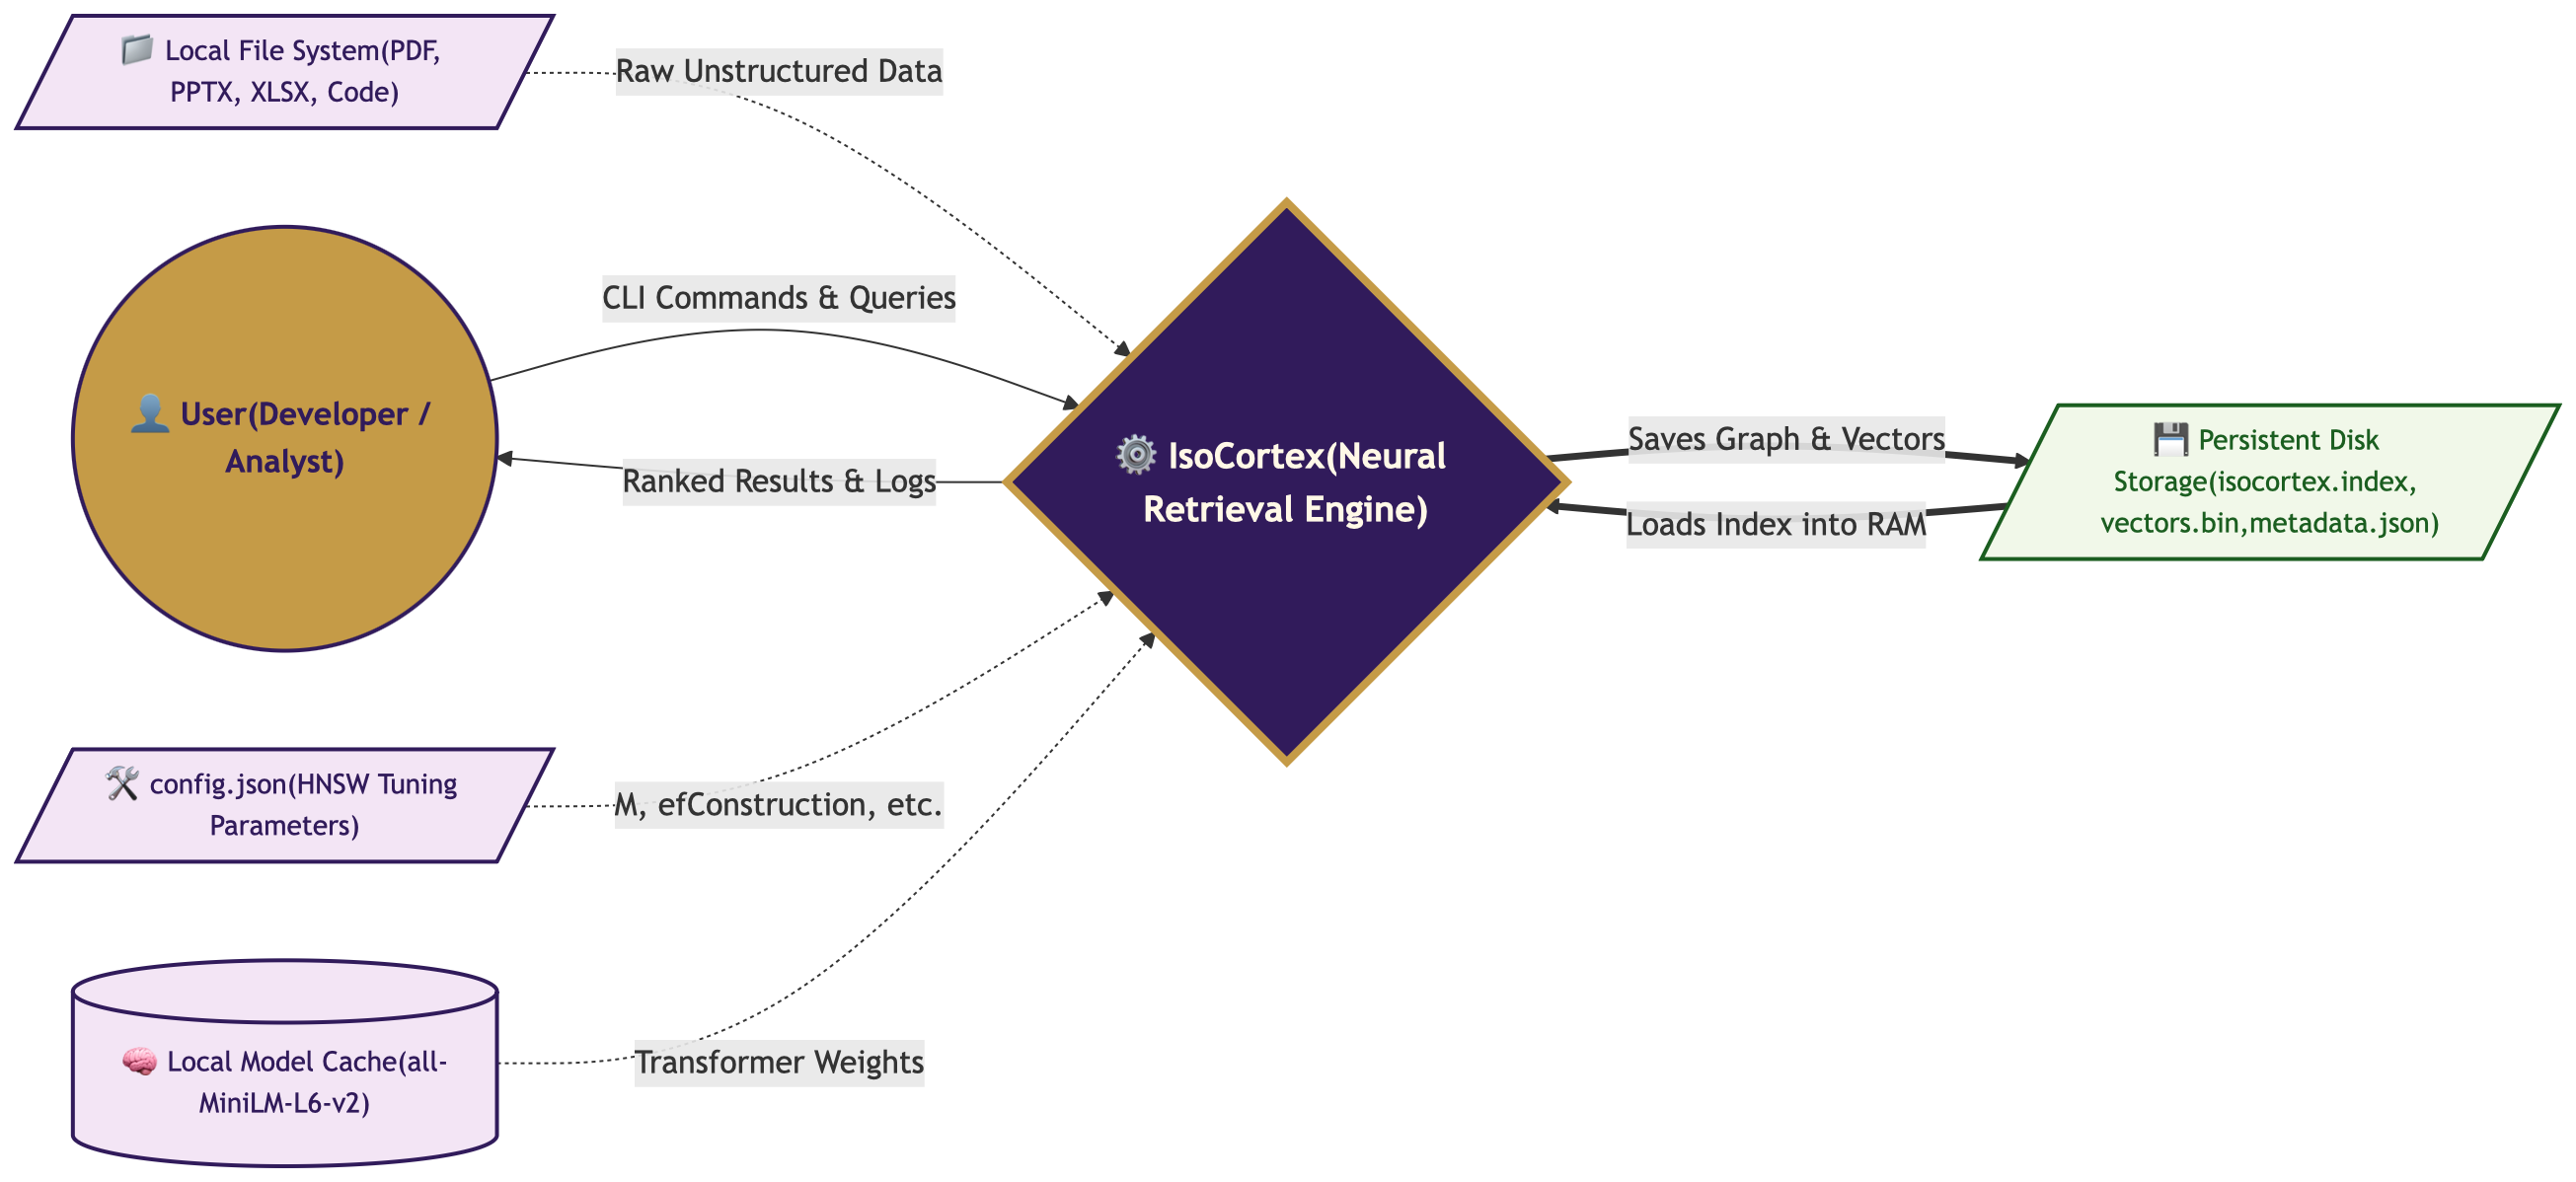
\includegraphics[width=0.9\textwidth, keepaspectratio]{context_diagram.png} 
    \end{tcolorbox}
    \caption{\textit{High-Level Context Diagram of the IsoCortex System}}
    \label{fig:context_diagram}
\end{figure}

\subsection{UML Behavioral Diagrams}
The Use Case diagram captures the functional requirements from the perspective of the developer/analyst operating the CLI.

\begin{figure}[h!]
    \centering
    \textbf{\large \textcolor{ctPurple}{System Use Cases}}\par\vspace{0.2cm}
    \begin{tcolorbox}[standardbox, colback=white, colframe=ctGold, width=0.95\textwidth, halign=center, bottom=5pt, top=5pt]
        % INSTRUCTION: Upload your image and name it 'usecase_diagram.png'
        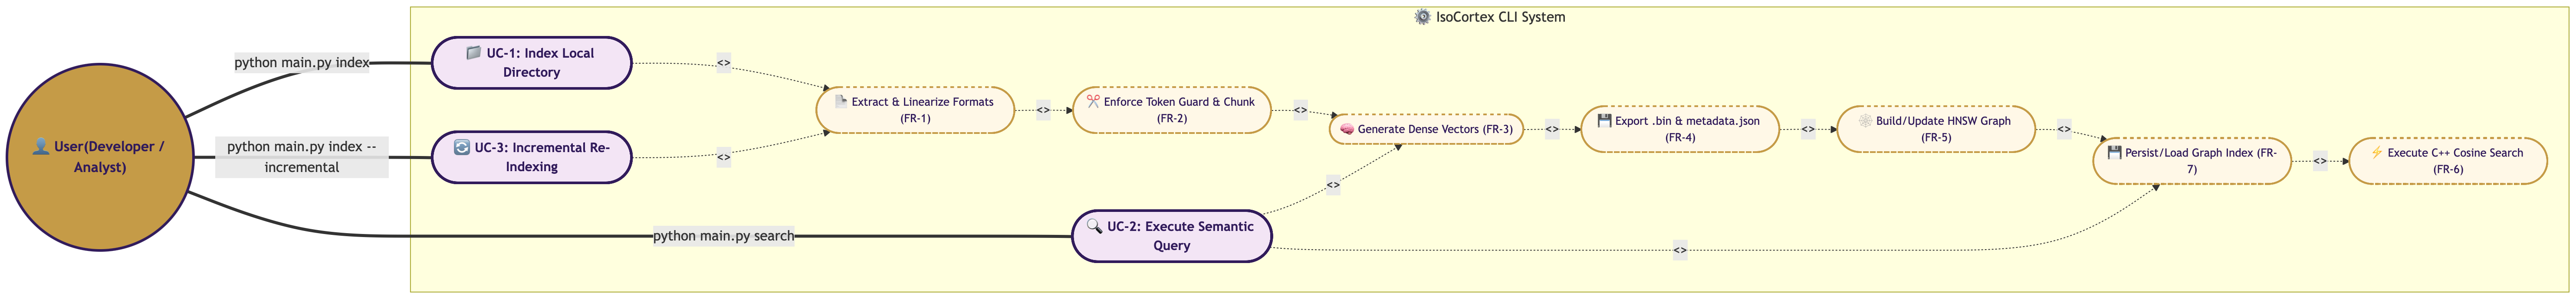
\includegraphics[width=0.9\textwidth, keepaspectratio]{usecase_diagram.png} 
    \end{tcolorbox}
    \caption{\textit{Use Case Diagram: Local User Interactions}}
    \label{fig:usecase_diagram}
\end{figure}

\subsection{UML Activity Diagram}
The Activity Diagram illustrates the step-by-step logic of the two-tier ingestion pipeline (Python Extraction $\rightarrow$ C++ HNSW Graph Build).

\begin{figure}[h!]
    \centering
    \begin{tcolorbox}[standardbox, colback=white, colframe=ctPurple, width=0.95\textwidth, halign=center, bottom=5pt, top=5pt]
        % INSTRUCTION: Upload your image and name it 'activity_diagram.png'
        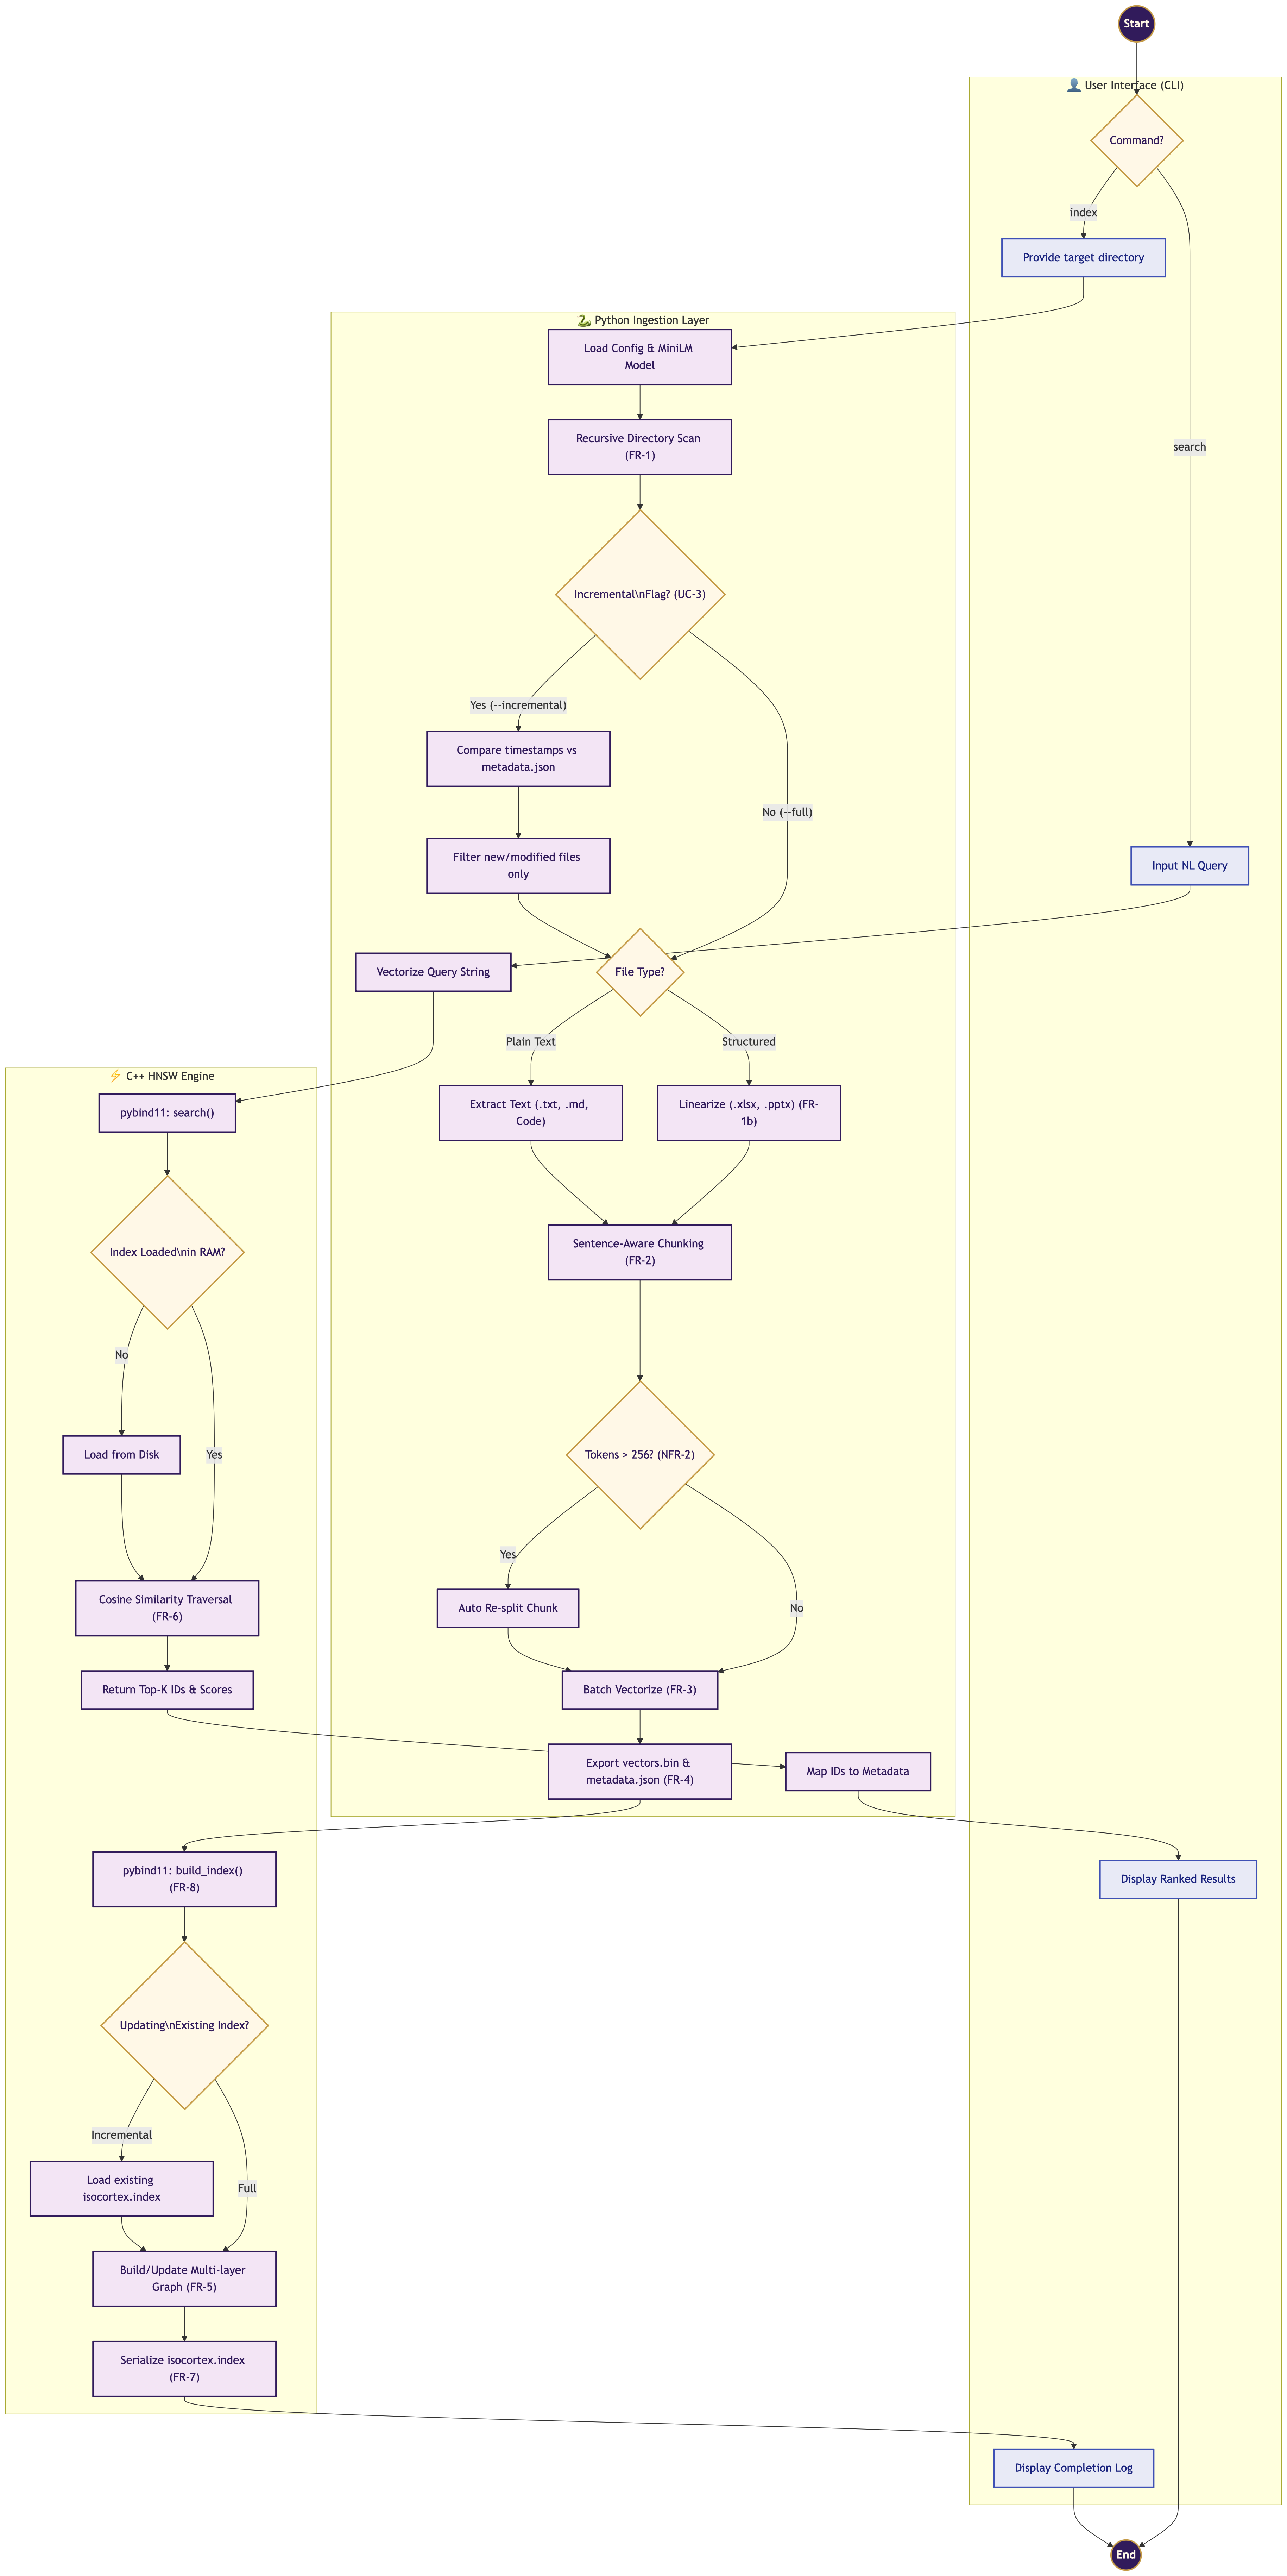
\includegraphics[width=0.9\textwidth, keepaspectratio]{activity_diagram.png}
    \end{tcolorbox}
    \caption{\textit{Activity Diagram: Ingestion and Indexing Workflow}}
    \label{fig:activity_booking}
\end{figure}

\end{document}